\section{Results}
\label{sec:results}

The recorded results are diverse, and incumbent with 
information. The honeypot records both time stamps, and 
interaction logs. Analysis of each will be handled separately 
in subsections \ref{sec:time_analysis} and 
\ref{sec:session_analysis}. 

It is worth noting that at this point in the project,
this section, along with the rest of the writing should
be considered to be work-in-progress.

\subsection{Statistical analysis of attack data}
\label{sec:time_analysis}

    The honeypot has been active since 12. of January
    2019, and until the 1. of March has logged 
    562.276 individual ssh attacks. 

    It was surprising that over 65 percent of attacks 
    originated in Ireland. A single IP address is the
    origin of 11.5 percent of attacks from Ireland 
    (see figure \ref{fig:ireland_breakdown})
    
    \begin{figure}
        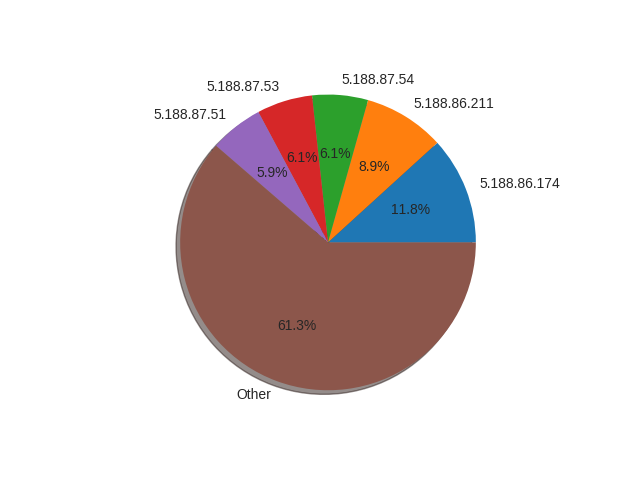
\includegraphics[width=0.8\textwidth]{src/images/ireland_breakdown.png}
        \caption{Attacks from Ireland broken down by source address}
        \label{fig:ireland_breakdown}
    \end{figure}

    A further investigation of the top-offender, 
    \texttt{5.188.86.174} reveals that this host
    is a tor exit node or relay \cite{tor}, which allows users
    to anonymize their internet activity. A nmap scan reveals
    a large number of services running on the host. As of \today
    there has been no attempt made to contact the host to notify
    them that their devices are complicit in potentially 
    illegal activity.


    If the rate of attempted attacks over time is plotted, 
    a pattern seems to start to emerge. (See figure \ref{fig:over_monday}
    for a plot of a typical monday)
    \begin{figure}
        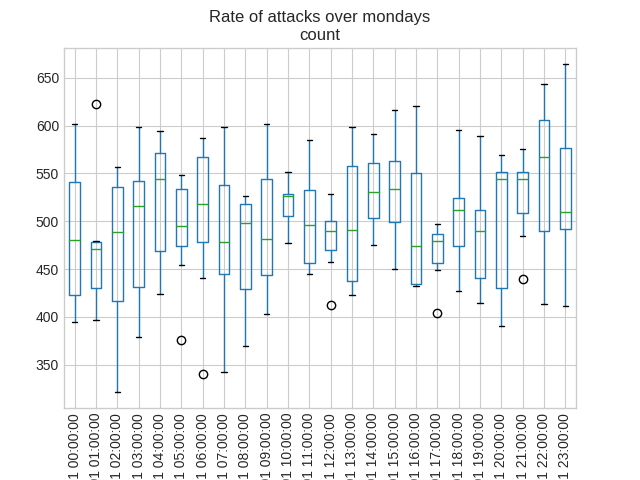
\includegraphics[width=0.8\textwidth]{src/images/OverMonday.png}
        \label{fig:over_monday}
    \end{figure}

    If the same done over the week (see figure \ref{fig:over_week}), there is a seemingly
    non-random pattern that can be discerned, in that 
    over the weekend, the rate becomes more varied.

    \begin{figure}
        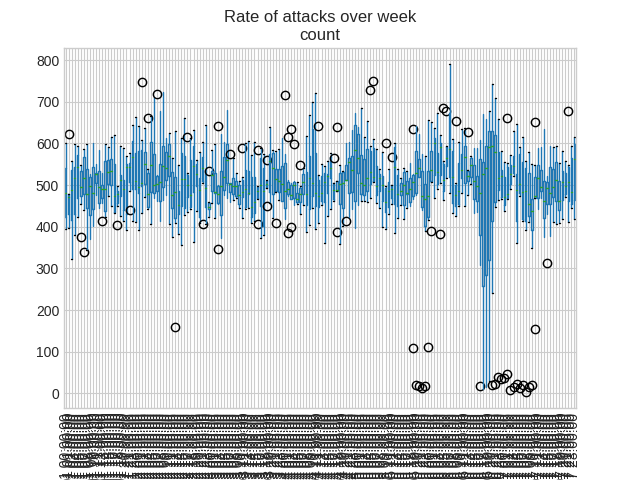
\includegraphics[width=0.8\textwidth]{src/images/week_unfiltered.png} 
        \label{fig:over_week}
    \end{figure}

    However, before any statistical analysis on the data is
    preformed, no conclusion should be drawn from apparent
    patterns.

\subsection{Session log analysis}
\label{sec:session_analysis}

    The cowrie honeypot also captures the actions of 
    the attacker, as well as the files which he attempts
    to download and run on what he thinks is a compromised
    server. 


    One of the more intriguing factors that a number of the
    attack logs show, is an attempt to access a command
    called \texttt{'\\gisdfoewrsfdf'}. A command that 
    has I do not know what does, and a search yields no
    definitive results to what this command or script is. 

    Amongst the other things that are attempted, 
    are wiping the \texttt{./ssh/authorized\_keys} file and
    inserting a key, presumably of another infected
    device. 

    Twice during the period of 12. January to 1. March, 
    did an attacker try to download, and start an IRC bot.

    